\section{Korunumlu Sistemler}

\begin{justify}
Newton yasası $F=ma$, birçok önemli ikinci mertebeden sistemin kaynağıdır. $x$ ekseni boyunca hareket eden ve doğrusal olmayan $F(x)$ kuvvetine maruz kalan $m$ kütleli parçacık için
\begin{equation}
m\ddot{x}=F(x)
\end{equation}
yazılır. Kuvvet hızdan ve zamandan bağımsızsa sönüm ya da dış zorlama yoktur.

$V(x)$ potansiyel enerji olsun ve
\begin{equation}
F(x)=-\frac{dV}{dx}
\end{equation}
ile tanımlansın. Böylece
\begin{equation}
m\ddot{x}+\frac{dV}{dx}=0
\end{equation}
olur. Denklem $\dot{x}$ ile çarpılırsa
\begin{equation}
\frac{d}{dt}\left[\frac{1}{2}m\dot{x}^{2}+V(x)\right]=0
\end{equation}
elde edilir. Dolayısıyla toplam enerji
\begin{equation}
E=\frac{1}{2}m\dot{x}^{2}+V(x)
\end{equation}
zaman boyunca sabittir. Korunan büyüklüğe sahip sistemlere korunumlu sistemler denir.
\end{justify}

\subsection*{Örnek 6.5.1}
\addcontentsline{toc}{subsection}{Örnek 6.5.1}

\begin{justify}
Korunumlu bir sistemin çekici sabit noktaya sahip olamayacağını gösterelim. $\mathbf{x}^{*}$ çekici sabit nokta olsaydı, çekim havzasındaki tüm noktalar aynı enerjiye sahip olurdu. Bu durumda $E(\mathbf{x})$ havza içinde sabit olurdu; bu da korunumlu sistem tanımıyla çelişir.
\end{justify}

\subsection*{Örnek 6.5.2}
\addcontentsline{toc}{subsection}{Örnek 6.5.2}

\begin{justify}
Kütlesi $m=1$ olan ve çift kuyulu potansiyel
\begin{equation}
V(x)=-\frac{1}{2}x^2+\frac{1}{4}x^4
\end{equation}
içinde hareket eden parçacığı ele alalım. Kuvvet
\begin{equation}
F=-\frac{dV}{dx}=x-x^3
\end{equation}
olduğundan
\begin{equation}
\ddot{x}=x-x^3
\end{equation}
yazılır. Vektör alanı
\begin{align}
\dot{x} &= y,\\
\dot{y} &= x-x^3
\end{align}
şeklindedir. Denge noktaları $(0,0)$ ve $(\pm1,0)$ noktalarıdır. Jacobian
\begin{equation}
A=\begin{pmatrix}0&1\\1-3x^2&0\end{pmatrix}
\end{equation}
olur. Orijin eyer noktasıdır; $(\pm1,0)$ noktaları merkez olarak öngörülür.

Enerji korunumu nedeniyle yörüngeler sabit enerji konturlarıdır:
\begin{equation}
E=\frac{1}{2}y^2-\frac{1}{2}x^2+\frac{1}{4}x^4=\text{sabit}.
\end{equation}
Faz portresi Şekil~\ref{fig:6-5-1}'de, fiziksel çift kuyu yorumu Şekil~\ref{fig:6-5-2}'de gösterilecektir.
\begin{figure}[H]
\centering
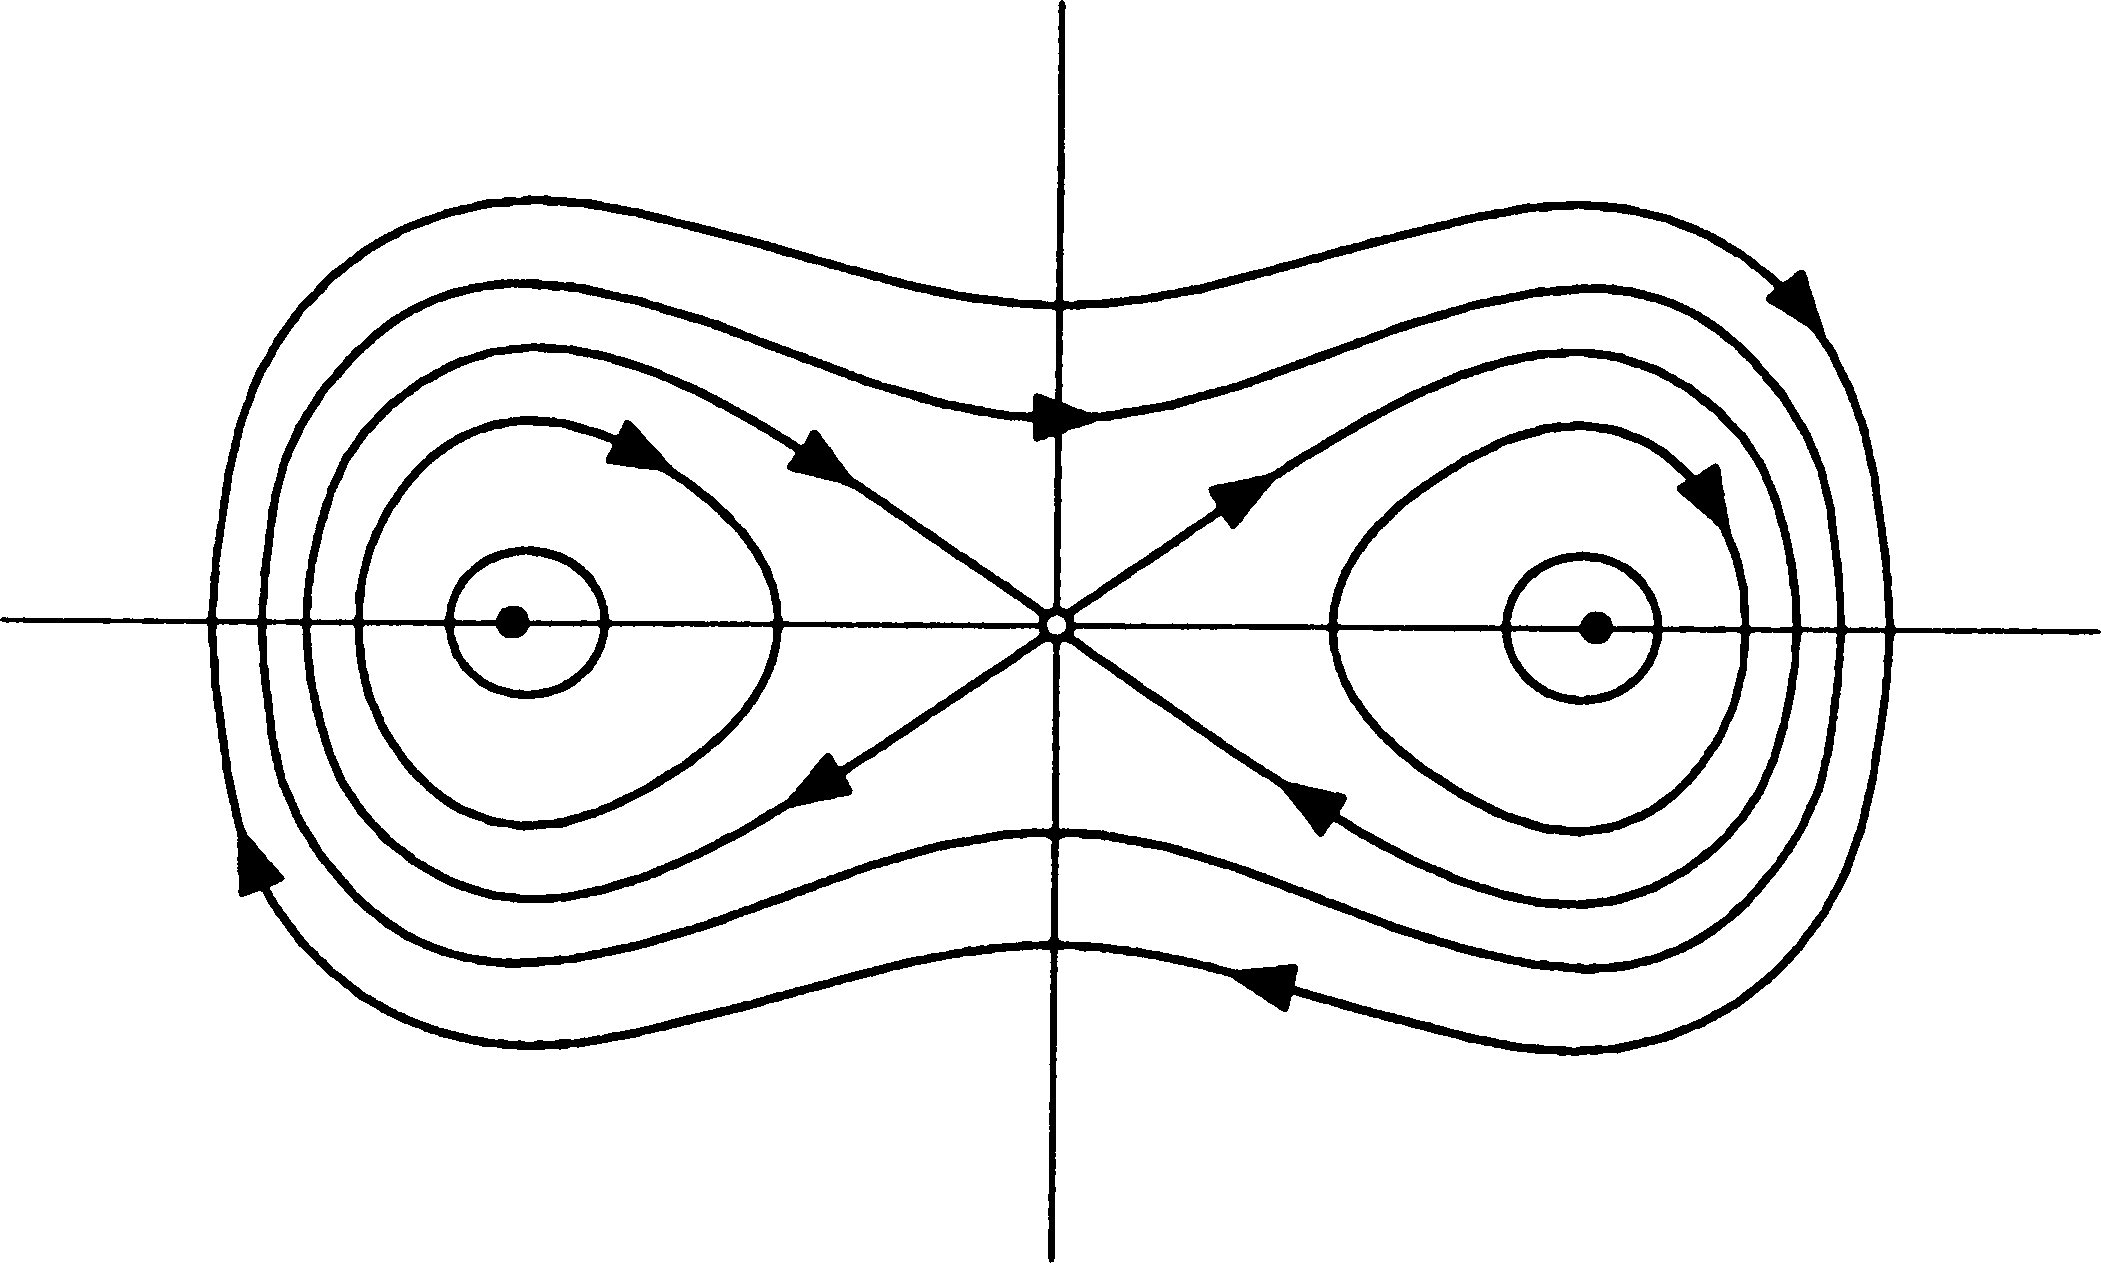
\includegraphics[width=0.82\textwidth]{images/Figures/figur-018.png}
\caption{Çift kuyulu potansiyel için faz portresi ve sabit enerji eğrileri.}
\label{fig:6-5-1}
\end{figure}
\begin{figure}[H]
\centering
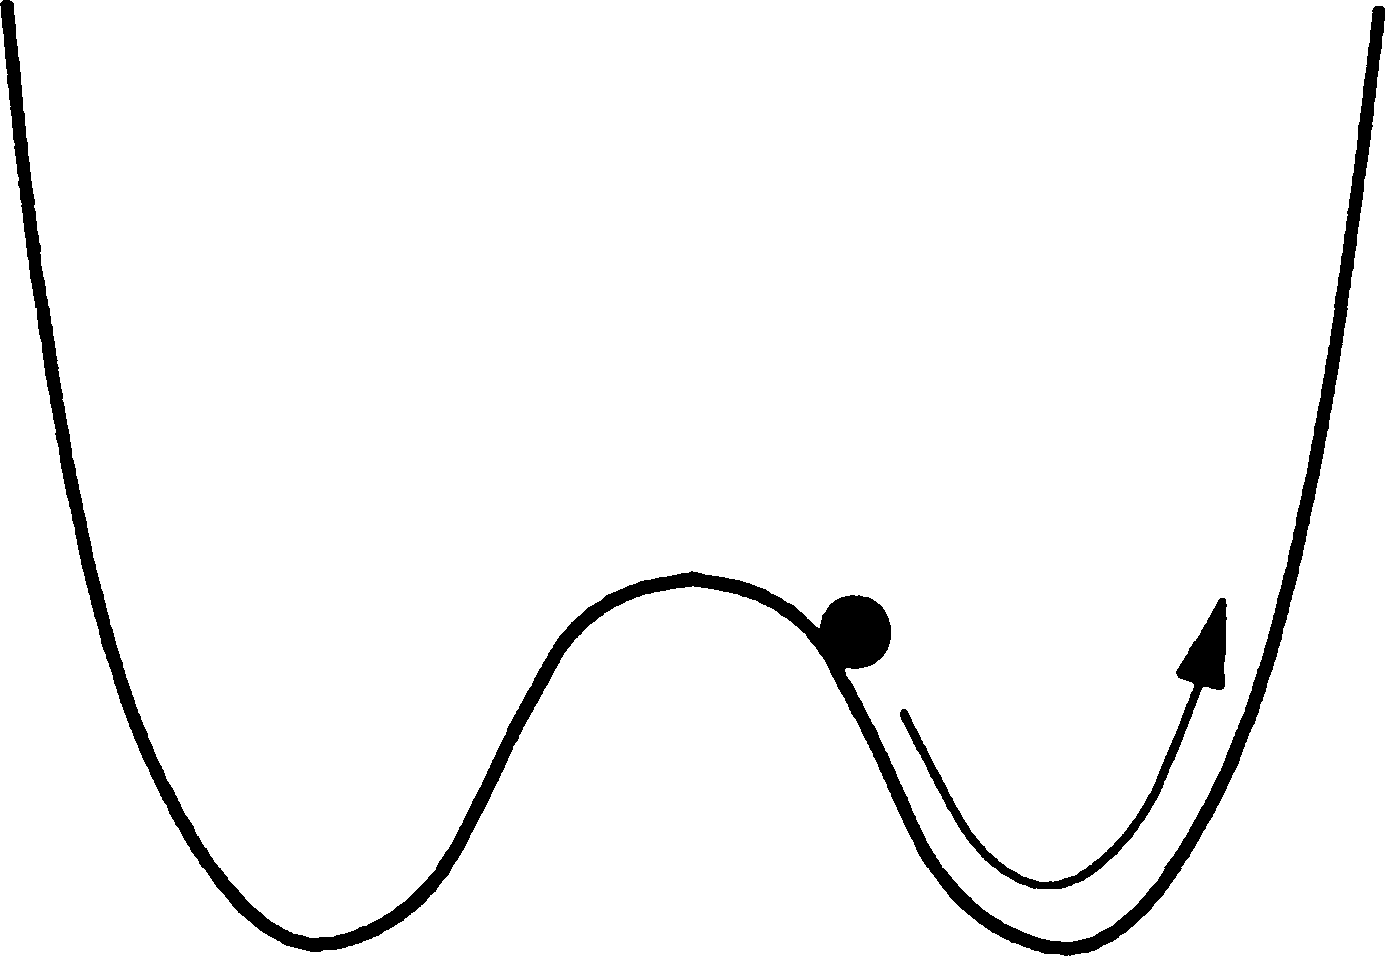
\includegraphics[width=0.82\textwidth]{images/Figures/figur-017.png}
\caption{Çift kuyulu potansiyelde parçacığın fiziksel hareketi.}
\label{fig:6-5-2}
\end{figure}
\end{justify}

\subsection*{Örnek 6.5.3}
\addcontentsline{toc}{subsection}{Örnek 6.5.3}

\begin{justify}
Örnek 6.5.2 için enerji fonksiyonu $E(x,y)$'nin grafiği enerji yüzeyi olarak adlandırılır (Şekil~\ref{fig:6-5-3}). Yerel minimumlar faz düzleminde merkezlere karşılık gelir.
\begin{figure}[H]
\centering
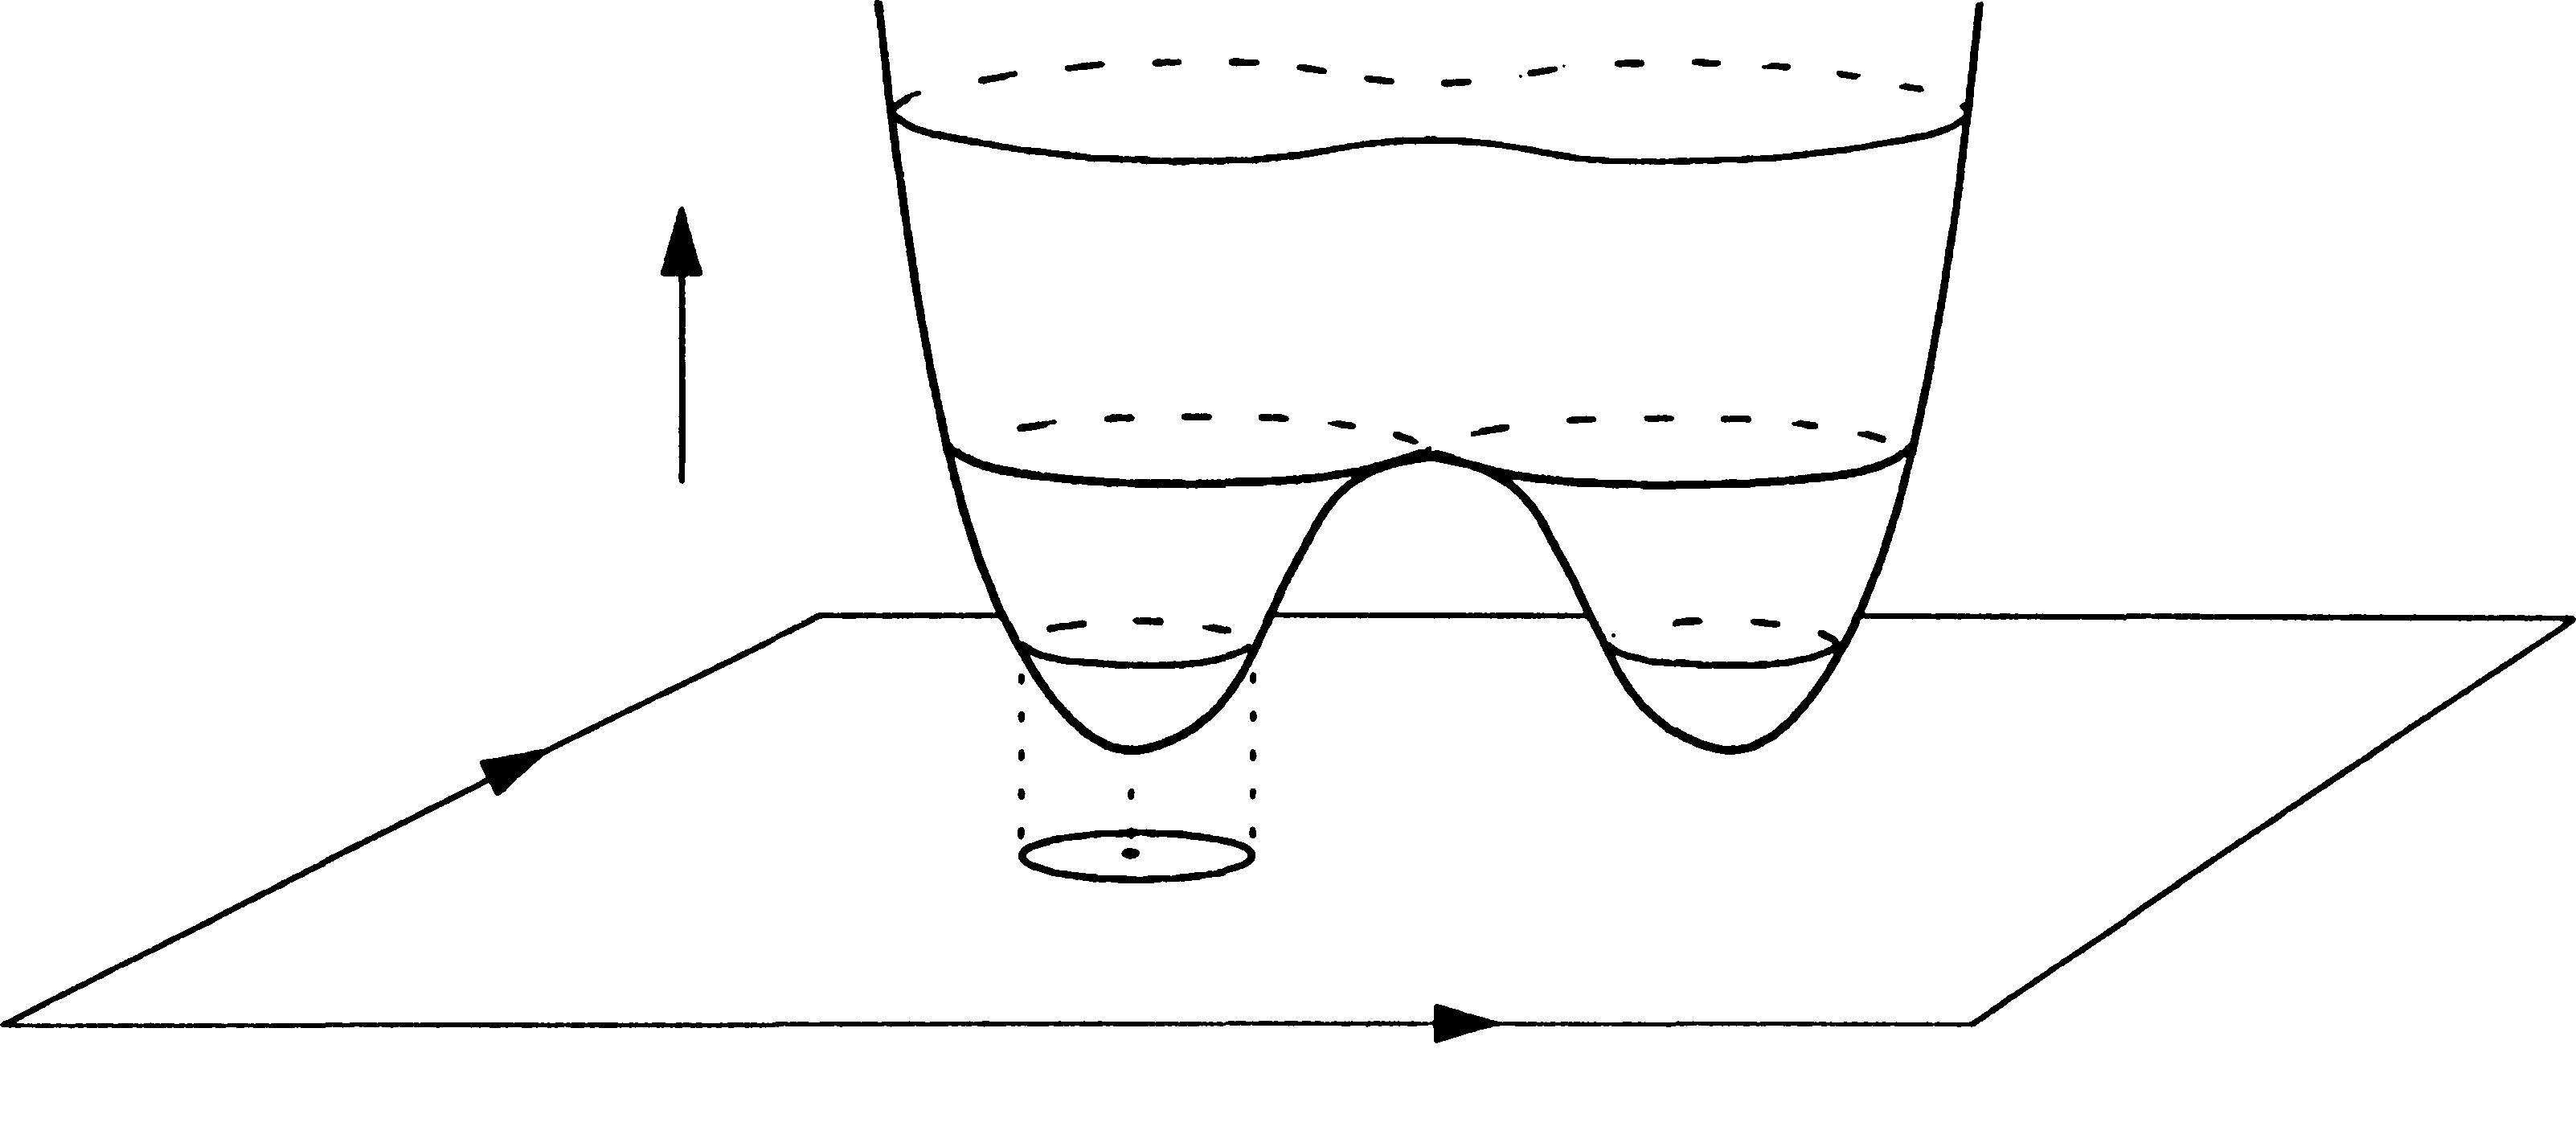
\includegraphics[width=0.82\textwidth]{images/Figures/figur-019.png}
\caption{Örnek 6.5.2 için enerji yüzeyi.}
\label{fig:6-5-3}
\end{figure}
\end{justify}

\subsection*{Doğrusal Olmayan Merkezler}
\addcontentsline{toc}{subsection}{Doğrusal Olmayan Merkezler}

\begin{justify}
Korunumlu sistemlerde merkezler daha dayanıklıdır; çünkü yörüngeler enerji konturları üzerinde kalır. Eğer izole bir sabit nokta $\mathbf{x}^{*}$, korunan büyüklük $E(\mathbf{x})$ için yerel minimum ise, $\mathbf{x}^{*}$ noktasına yeterince yakın tüm yörüngeler kapalıdır. Bu nedenle $\mathbf{x}^{*}$ doğrusal olmayan bir merkezdir.
\end{justify}

\newpage